\newpage
\section{Turn Up the Volume!}
\begin{teachingnote}
Supplies: tape, scissors, and copies of the net.
\end{teachingnote}
In this activity, we will investigate formulas for area and
volume.


\begin{prob}
Explain how the following picture ``proves'' that the area of a right
  triangle is one half of the base times the height.
\[
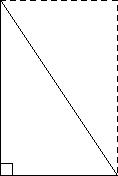
\includegraphics{../graphics/pbpAreaRight.pdf}
\]
\end{prob}

\begin{prob}
``Shearing'' is a process where you take a shape, cut it into thin parallel strips, 
and then move the strips in a direction parallel to the strips to make a new shape.  
By Cavalieri's principle:\index{Cavalieri's principle}
\begin{quote}
Shearing parallel to a fixed direction does not change the $n$-dimensional measure of an object.
\end{quote}
What is this saying?
\end{prob}

\begin{prob}
Building on the first two problems, explain how the following picture
  ``proves'' that the area of any triangle is one half of the base times the
  height.
\[
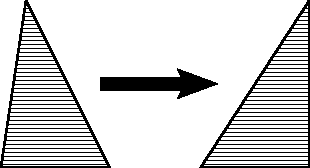
\includegraphics{../graphics/pbpShearTri.pdf}
\]
\end{prob}

\begin{prob}
Explain how to use a picture to ``prove'' that a triangle of a given
  area could have an arbitrarily large perimeter.
\end{prob}
\vspace{.25in}

\begin{prob}
Shearing is a special case of Cavalieri's principle, which, in two dimensions, is stated as follows:  
\begin{quote}
Suppose two regions in a plane are contained between two parallel lines.  If every line parallel to the given lines intersects the two regions in equal lengths, then the regions have equal area.  
\end{quote}
Give an intuitive argument explaining why Cavalieri's principle is true.
\end{prob}

\begin{prob}
State Cavalieri's principle in three dimensions.  
\end{prob}
\vspace{.25in}


%
%\begin{prob}
%Sketch a net for a right pyramid of height $2''$ with a $2'' \times
%2''$ square base. Share your sketch with your neighbor---does it look
%OK?
%\end{prob}
%
%
%\begin{prob}
%Give detailed diagrams that show that a cube can be constructed from
%three equal pyramids.
%\end{prob}

\begin{prob}
Cut out the provided net.  Then fold it and tape it to create a square-based pyramid.  With your neighbors, show that three such square-based pyramids can form a cube.  
\end{prob}
\begin{teachingnote}
Here is the net
\[
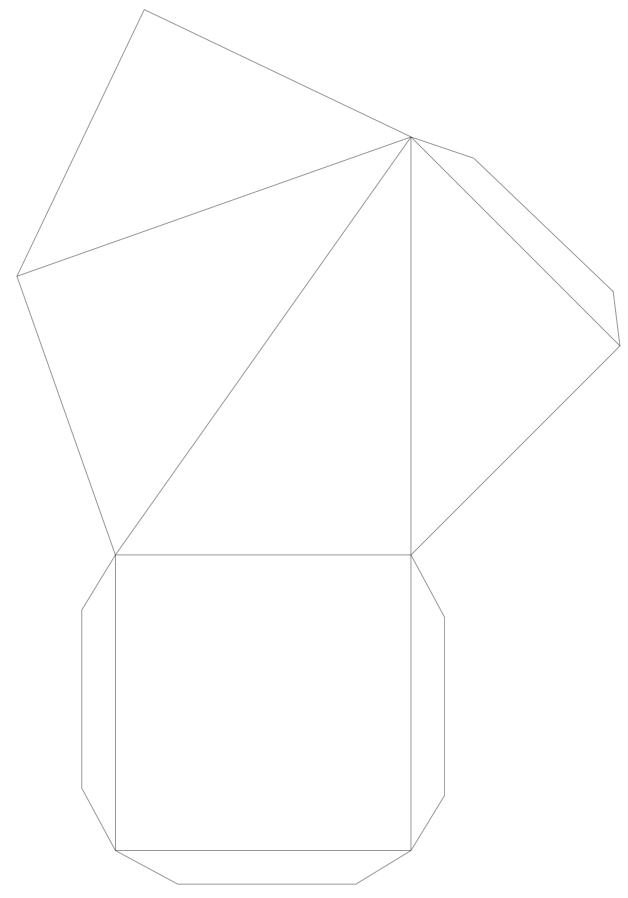
\includegraphics[angle=90,scale=0.7]{../graphics/rightPyramid}
\]
\end{teachingnote}

\begin{prob}
Use your work above to derive a formula for the volume of a
right pyramid with a square base. The formula should be in terms of
the side length of the square base.
\end{prob}

\begin{prob}
Use Cavalieri's principle to explain the formula for \textbf{every} pyramid with an $s\times s$ square base of height $s$ in terms of $s$.  Be sure to describe how this formula is different from the previous one.  
\end{prob}

\begin{prob}
Provide an informal explanation of a volume formula for any pyramid-like object with a base of area $B$ and height $h$.  Be sure to describe what you mean by ``pyramid-like'' and whether your formula works for a cone.  
\end{prob}

\begin{prob}
% \standard{8.G.9}
In this problem you derive the formula for the volume of a sphere of radius $r$.\standardhs{G-GMD.1}\standardhs{G-GMD.2}   The figures below shows a half-sphere of radius $r$ alongside a cylinder of radius $r$ and height $r$ with a cone of radius $r$ and height $r$ removed.
\[
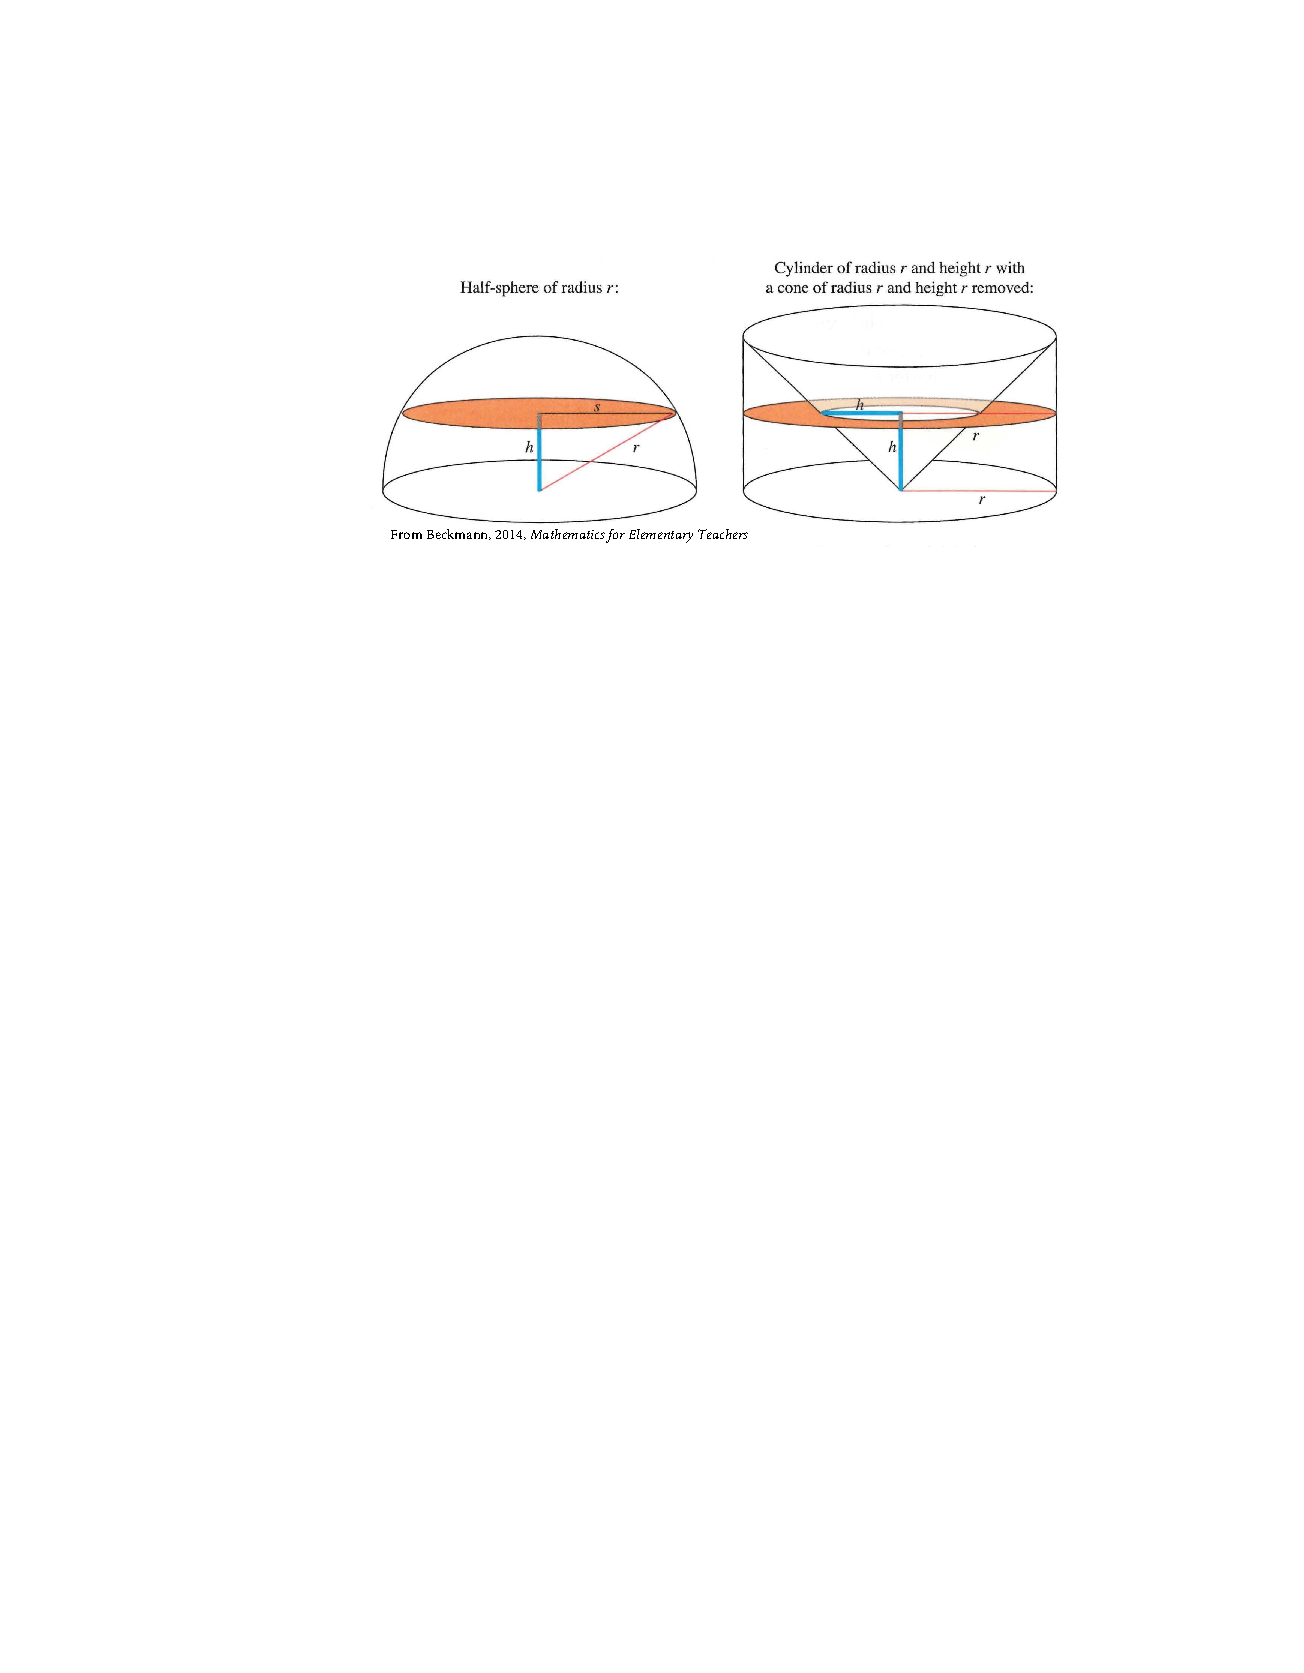
\includegraphics[scale=1.1]{../graphics/sphereVolume}
\]
Think of $r$ as fixed, and think of $h$ as the varying height of a cross section.  The (hard to read) $s$ is the radius of the cross-section of the sphere.  
\begin{enumerate}
\item The heights of the cylinder and the cone are not $h$.  What are their heights?  
\item What is $h$?  Explain why the several values labeled $h$ are indeed equal.   
\item Draw and label an ``aerial view'' of the cross sections.   
\item Explain why the cross-sections at height $h$ have the same area.  
\item Use the formula for the volume of a cone and Cavalieri's principle to derive a formula for the volume of a sphere of radius $r$.  
\end{enumerate}
\fixnote{Replace graphic?}
\end{prob}
